\documentclass[12pt, a4paper]{article}
\usepackage[T1]{fontenc}
\usepackage[utf8]{inputenc}
\usepackage[polish]{babel}
\usepackage[margin=2.5cm]{geometry}
\usepackage{array}
\usepackage{tabularx}
\usepackage{setspace}
\usepackage{verbatim}
\usepackage{amsmath}
\usepackage{amssymb}
\usepackage[hidelinks]{hyperref}
\usepackage{tocloft}
\usepackage{float}
\usepackage{listings}
\usepackage{graphicx}
\renewcommand{\cftsecleader}{\cftdotfill{\cftdotsep}}

\onehalfspacing

\lstset{
    basicstyle=\ttfamily\small,
    breaklines=true,
    frame=single,
    captionpos=b,
    extendedchars=true,
    keepspaces=true,
    columns=fixed,
    commentstyle=\normalfont\ttfamily,
    showstringspaces=false,
    literate={ą}{{\k{a}}}1 {ć}{{\'c}}1 {ę}{{\k{e}}}1 {ł}{{\l{}}}1 {ń}{{\'n}}1 {ó}{{\'o}}1 {ś}{{\'s}}1 {ź}{{\'z}}1 {ż}{{\.z}}1 {Ą}{{\k{A}}}1 {Ć}{{\'C}}1 {Ę}{{\k{E}}}1 {Ł}{{\L{}}}1 {Ń}{{\'N}}1 {Ó}{{\'O}}1 {Ś}{{\'S}}1 {Ź}{{\'Z}}1 {Ż}{{\.Z}}1
}

\title{\vspace*{3cm} \textbf{Dokumentacja Projektowa JAVA \\ System Wizualizacji Grafów}}
\author{Mateusz Bombola \\ Kajetan Karwacki}
\date{\today}

\begin{document}

\maketitle
\thispagestyle{empty}

\newpage
\tableofcontents
\newpage

\section{Wstęp i Cel Projektu}
Celem projektu jest okienkowa aplikacja w języku Java (wykorzystująca bibliotekę Swing), służąca do interaktywnej wizualizacji topologii grafów planarnych na płaszczyźnie 2D. Program pełni rolę graficznego interfejsu użytkownika (GUI) oraz orkiestratora, który integruje się z zewnętrznym silnikiem obliczeniowym w języku C. Aplikacja pobiera zdefiniowane krawędzie, wywołuje program w C w celu uzyskania zoptymalizowanych współrzędnych węzłów, a następnie płynnie renderuje i pozwala na modyfikację wygenerowanego układu.

\section{Specyfikacja Funkcjonalna}

\subsection{Realizowane Funkcje}
\begin{itemize}
    \item Wczytywanie struktury grafu z plików tekstowych (.txt).
    \item Interaktywne renderowanie układu z dynamicznym kolorowaniem krawędzi (gradient od zieleni do czerwieni) na podstawie wczytanych wag.
    \item Wybór algorytmu obliczeniowego (Fruchterman-Reingold lub Tutte Embedding) z poziomu interfejsu graficznego.
    \item Swobodne manipulowanie kamerą: przybliżanie i oddalanie (zoom) za pomocą kółka myszy oraz przesuwanie widoku (panning).
    \item Edycja układu w czasie rzeczywistym poprzez ręczne przeciąganie wierzchołków metodą „Drag \& Drop” oraz precyzyjną edycję w panelu właściwości.
    \item Zapis wyliczonych współrzędnych do pliku .txt oraz eksport widoku obszaru roboczego do pliku graficznego (.png).
\end{itemize}

\subsection{Interfejs Użytkownika (GUI)}
Program działa w trybie okienkowym. Składa się z górnego paska narzędziowego (Menu) obsługującego wejście/wyjście plików, centralnego płótna renderującego (\texttt{GraphPanel}) oraz prawego panelu bocznego, który skupia kontrolki sterujące silnikiem obliczeniowym, pola edycyjne zaznaczonego węzła i opcje wyświetlania (włączanie/wyłączanie etykiet oraz wag).

\section{Architektura i Implementacja}

\subsection{Podział na Moduły}
Aplikacja opiera się na podejściu obiektowym i dzieli się na następujące klasy:
\begin{itemize}
    \item \textbf{\texttt{GraphApp}}: Klasa główna odpowiadająca za konstrukcję głównego okna (\texttt{JFrame}), układ komponentów, walidację interakcji oraz zarządzanie zintegrowanym procesem C.
    \item \textbf{\texttt{GraphPanel}}: Silnik renderujący (\texttt{JPanel}). Nadpisuje metodę \texttt{paintComponent} w celu rysowania grafiki wektorowej za pomocą \texttt{Graphics2D} oraz obsługuje nasłuchiwacze zdarzeń myszy.
\end{itemize}

\subsection{Struktury Danych}
Dane topologiczne przechowywane są przy pomocy lekkich klas:
\begin{itemize}
    \item \textbf{\texttt{Node}}: Przechowuje identyfikator (\texttt{id}) oraz pozycje \texttt{x} i \texttt{y} (zmiennoprzecinkowe) dla każdego węzła. Węzły mapowane są w słowniku \texttt{Map<Integer, Node>}.
    \item \textbf{\texttt{Edge}}: Definiuje połączenie między dwoma wierzchołkami (\texttt{u}, \texttt{v}) wraz z przypisaną mu wagą (\texttt{weight}). Krawędzie przechowywane są w kolekcji \texttt{List<Edge>}.
\end{itemize}

\section{Kluczowe Mechanizmy i Integracja}

\subsection{Współpraca z silnikiem C}
Program wykorzystuje obiekt \texttt{ProcessBuilder} do natywnego uruchomienia wygenerowanego pliku \texttt{graph\_layout.exe}. 
Dla zapewnienia bezproblemowej pracy w strukturze projektu, aplikacja używa dynamicznego radaru ścieżek – przeszukuje predefiniowaną lista folderów (m.in. \texttt{Algorytm c/pliki\_zrodlowe\_2\_grupy/}). Komenda uruchomienia budowana jest z uwzględnieniem specyfiki drugiej grupy (przekazywanie ścieżki wejściowej bez flagi oraz ewentualne użycie flagi \texttt{-a} dla algorytmu Tutte'a).

\subsection{Dynamiczne Skalowanie Współrzędnych}
Algorytmy dystansowe mogą zwracać wartości znormalizowane do ułamków dziesiętnych. Przed rzutowaniem pozycji na piksele (\texttt{int}), Java analizuje przestrzeń (\texttt{getDynamicScale()}). Gdy najwyższa wartość współrzędnej jest mniejsza od zdefiniowanego progu (15 jednostek), aplikacja stosuje do rysowania globalny mnożnik 150.0. Eliminuje to błąd numeryczny objawiający się „zapadnięciem” grafu.

\subsection{Automatyczne Centrowanie}
Metoda \texttt{resetView()} iteruje po załadowanych węzłach w celu odnalezienia wartości \texttt{minX}, \texttt{maxX}, \texttt{minY} oraz \texttt{maxY}. Z uzyskanej obwiedni wyliczany jest środek ciężkości grafu, a wartości przesunięcia kamery (\texttt{px}, \texttt{py}) są odpowiednio korygowane. Dzięki temu układ po obliczeniach zawsze wyświetlany jest dokładnie pośrodku ekranu użytkownika, niezależnie od bazowych wartości wynikowych.

\section{Obsługa Plików i Błędy}
Moduł I/O obsługuje ładowanie i zapis plików tekstowych, odczytując linie i weryfikując poprawność długości wprowadzonych danych.

\subsection{Reakcje na błędy (Kody wyjątkowe)}
Aplikacja zabezpiecza działanie systemu i informuje użytkownika poprzez wyskakujące okna (\texttt{JOptionPane}):
\begin{table}[H] 
\centering
\large 
\renewcommand{\arraystretch}{1.5} 
\begin{tabular}{|p{4.5cm}|p{10.5cm}|}
\hline
\textbf{Sytuacja Wyjątkowa} & \textbf{Reakcja Systemu Java} \\ \hline
Brak danych krawędzi & Blokada wywołania silnika C i komunikat „Najpierw wczytaj strukturę krawędzi!”. \\ \hline
Nieznalezienie pliku EXE & Włączenie okna \texttt{JFileChooser} pozwalającego użytkownikowi wskazać ręcznie lokalizację silnika. \\ \hline
Błąd w module C & Przechwycenie kodu powrotu oraz wiadomości ze strumienia błędów (\texttt{ErrorStream}) i wyświetlenie alertu „Awaria w C”. \\ \hline
\end{tabular}
\end{table}

\section{Dokumentacja Graficzna Interfejsu}

\begin{figure}[H]
    \centering
    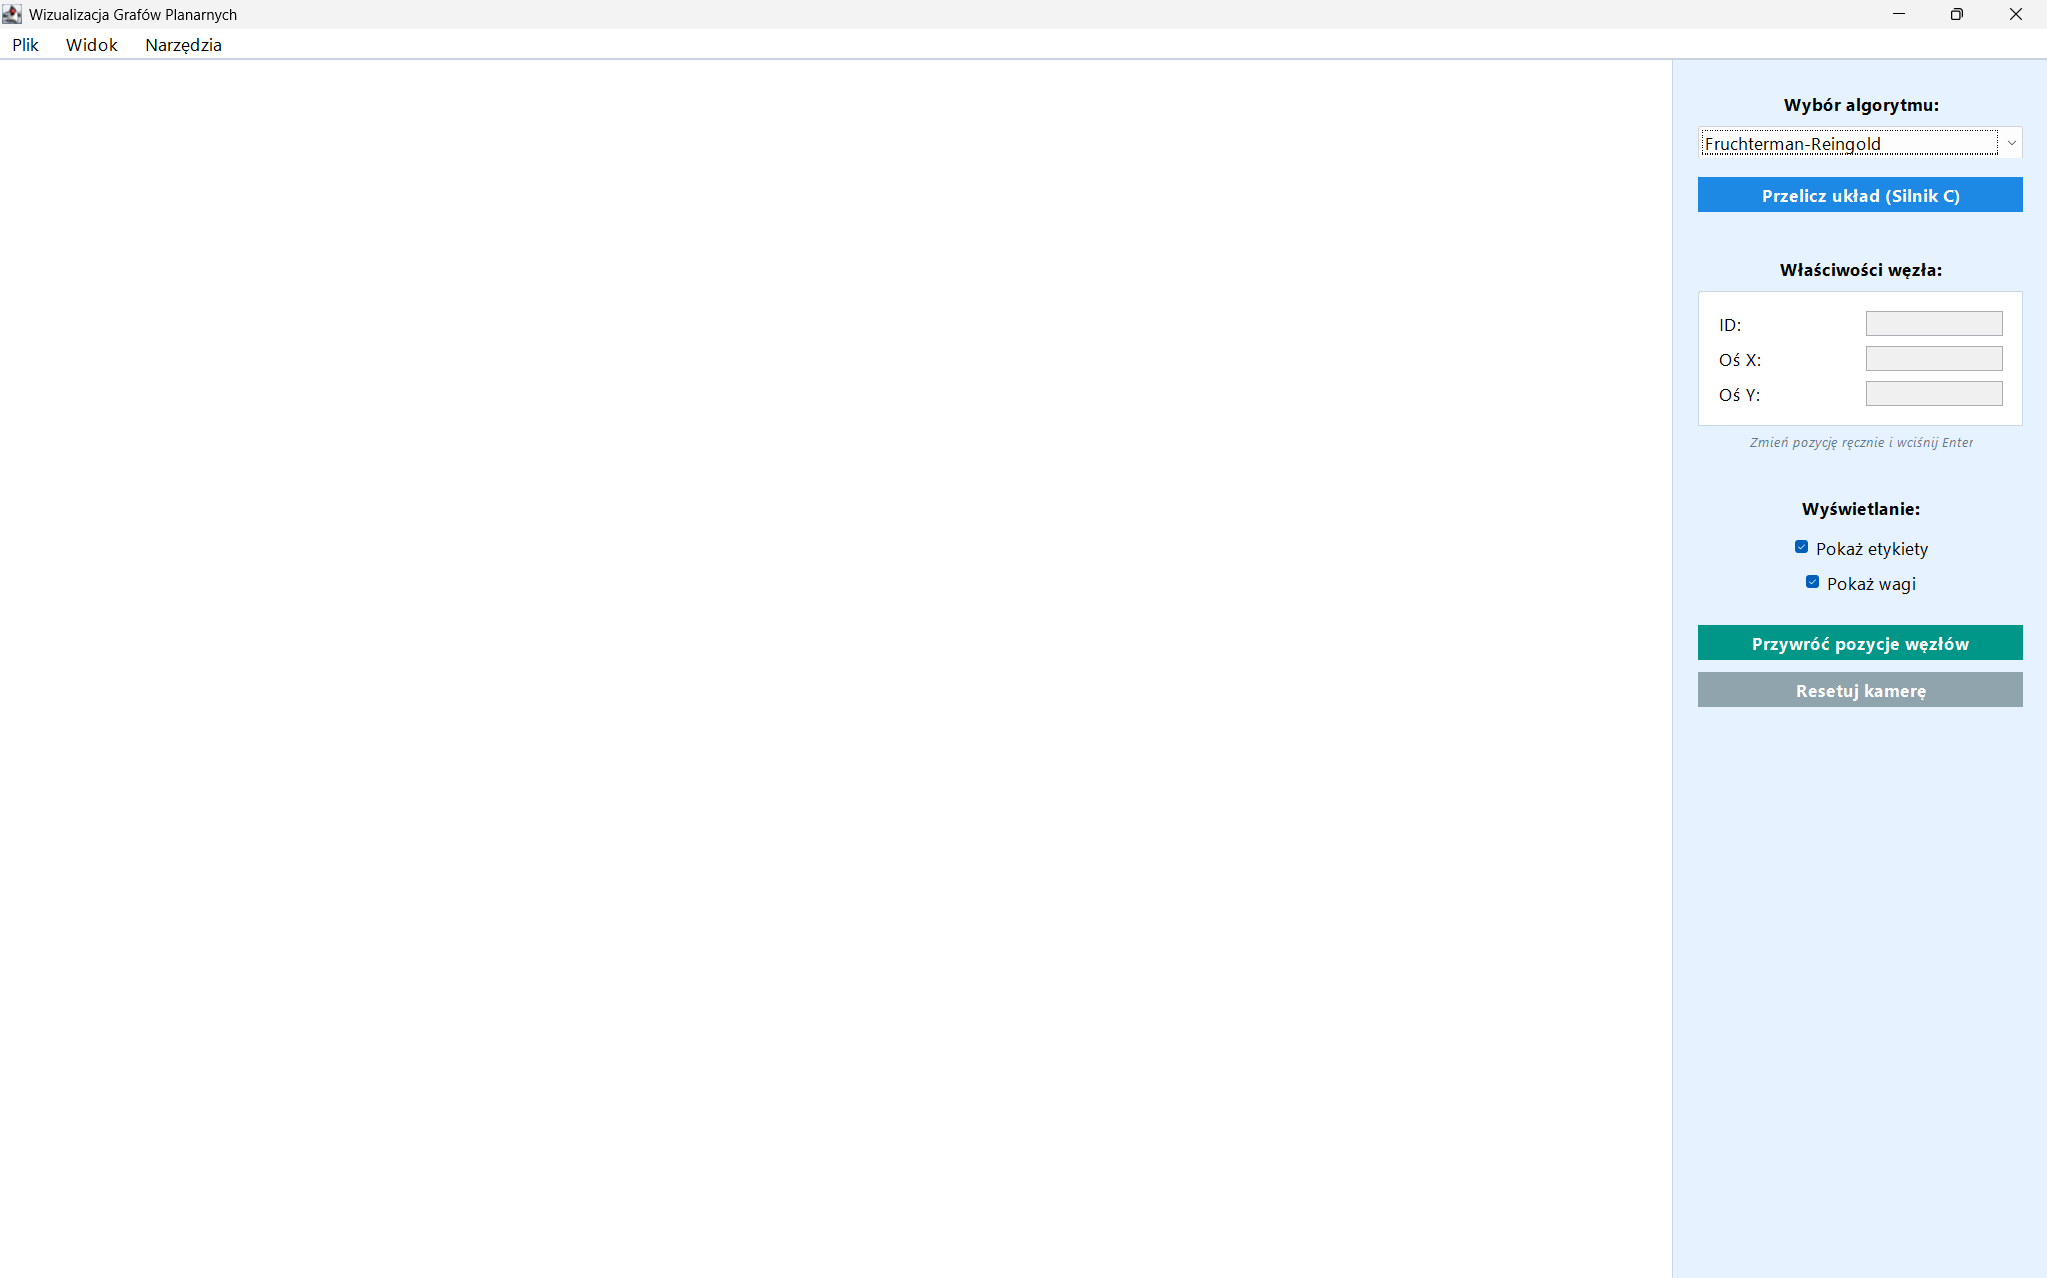
\includegraphics[width=0.8\textwidth]{a1.png}
    \caption{Główne okno programu przed załadowaniem struktury grafu}
\end{figure}

\begin{figure}[H]
    \centering
    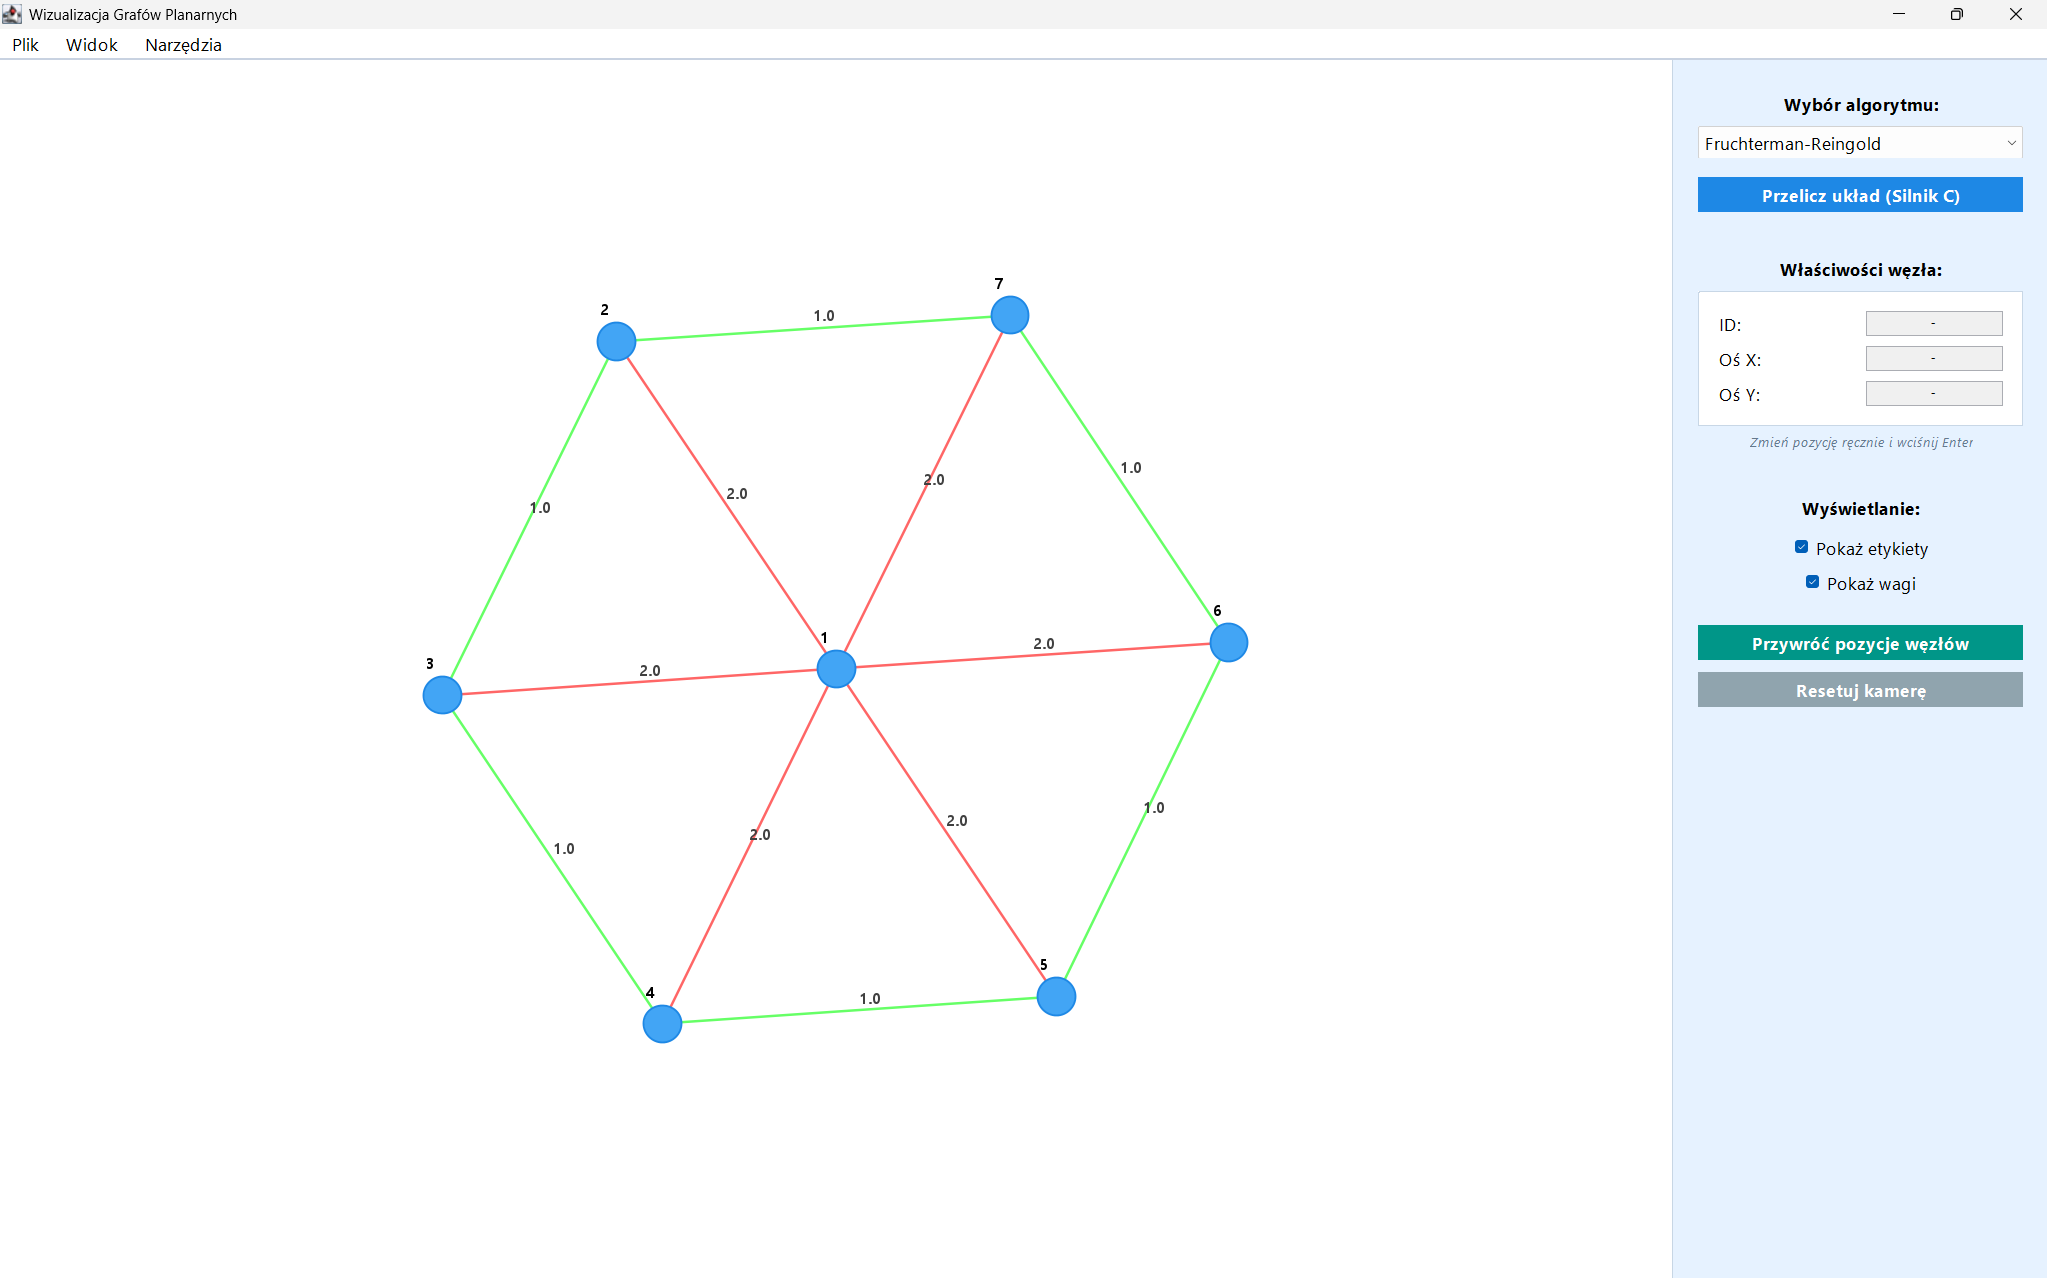
\includegraphics[width=0.8\textwidth]{a2.png}
    \caption{Wycentrowany układ wierzchołków uzyskany po wykonaniu obliczeń przez silnik C}
\end{figure}

\end{document}